\documentclass{article}
\usepackage{etoolbox}
\usepackage{graphicx}

\ifdef{\myoutput}{}{\def\myoutput{concept}}
\ifdef{\myversion}{}{\def\myversion{1}}

\usepackage[output=\myoutput
,numberofversions=4
,version=\myversion
,seed=4
,randomizequestions=true
,randomizeanswers=true
,writeRfile=true
]{mcexam}

\usepackage[margin=0.95in]{geometry}
\usepackage{multicol}

\usepackage{fancyhdr,lastpage}
\pagestyle{fancy}
\fancyhf{}
\renewcommand{\headrulewidth}{1pt} 
\renewcommand{\footrulewidth}{1pt}
\lfoot{\mctheversion}
\rfoot{Page \thepage\ of \pageref{LastPage}}
\lhead{Quiz 3.3 Version \fbox{\myversion} \\ MAT 2000: Introduction to Statistics}
\rhead{Name Print): \hspace{2.5 in}}

\usepackage{calc}
\renewenvironment{setmcquestion}
{\begin{minipage}[t]{\linewidth-\labelwidth}}
	{\end{minipage}\par}
	
\renewenvironment{setmcquestioninstruction}
{\begin{minipage}{\textwidth}}
	{\end{minipage}}
	
\renewenvironment{setmcanswers}{}{}
\setlist[setmcquestions]{label=\mcquestionlabelfmt{*}.
	,ref=\mcquestionlabelfmt{*}
	,itemsep=0.5\baselineskip
	,topsep=1\baselineskip
}

\renewcommand\mcversionlabelfmt[1]{\arabic{#1}}

%\mcifoutput{exam}{
%	\AtEndDocument{\ifodd\value{page}
%		\newpage\thispagestyle{empty}\hbox{This page intentionally left blank.}\newpage\thispagestyle{empty}\hbox{}
%		\else
%		\newpage\thispagestyle{empty}\hbox{}
%		\fi}
%}

\raggedbottom

\begin{document}
	Circle the correct answer for each question.  If you're unsure, you can write numbers 1, 2, 3, etc. next to the choices to get partial credit.\\[.5cm]
	\begin{mcquestions}
		\question The following 19 test scores are based on a random sample of final exam scores (sorted in increasing order) for the population of students who took an elementary statistics course at a large university over a 5 year period:
		\begin{tabular}{ccccccccccccccccccc}
			61 &  65 &  69  & 70  & 71 &  73  & 75 &  77 &  77 &  82  & 82 &  83 &  84 &  85 &  86 &  89 &  92  & 92 &  94
		\end{tabular}
		Suppose the largest test score in the sample changed from a 94 to a 90. Describe how each of the following statistics would change.
		The median would \_\_\_(1)\_\_\_.
		The mean would \_\_\_(2)\_\_\_.
		The standard deviation would \_\_\_(3)\_\_\_.
		
		\begin{mcanswerslist}
			\answer decrease, decrease, decrease
			\answer remain the same, decrease, increase
			\answer[correct] remain the same, decrease, decrease
			\answer decrease, increase, remain the same			
		\end{mcanswerslist}
		
		\question Suppose a population of test scores is skewed right. What would be the shape of the sampling distribution for sample mean test scores from samples of 50 students?
		\begin{mcanswerslist}
			\answer Skewed right
			\answer Skewed left
			\answer[correct] Approximately normal
			\answer Unable to determine
		\end{mcanswerslist}
		
		\question If a bootstrap distribution of 1,000 sample medians was generated rather than 1,000 sample means, what would be the shape of the bootstrap distribution of sample medians?
		\begin{mcanswerslist}
			\answer Approximately normal
			\answer Skewed right
			\answer Skewed left
			\answer[correct] Unable to determine
		\end{mcanswerslist}
		
		\begin{mcquestioninstruction}
			Noxious weeds are invasive plants that quickly spread and deplete the soil of nutrients that are required for all aspects of farming and ranching. With much at stake, the state of Montana has hired a team of researchers to explore the issue. Researchers want to know the average number of noxious weeds per acre in North Central Montana. To do so, the researchers divided the area of interest into 1,000,000 acres and randomly selected 24 of these acres. For each selected acre, the noxious weeds were counted and removed. The sample mean was 103.47 weeds, and the sample standard deviation was 46.034 weeds.
		\end{mcquestioninstruction}
		
		\question What is the population of interest?
		\begin{mcanswerslist}
			\answer[correct] All acres in North Central Montana
			\answer The 24 selected acres in the sample
			\answer The true mean number of noxious weeds per acre in North Central Montana
			\answer The sample mean number of noxious weeds per acre
		\end{mcanswerslist}
		
		\question[follow] Below is the simulated bootstrap distribution of 1,000 sample means created from resampling the observed data.
		\begin{center}
			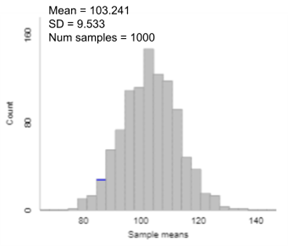
\includegraphics{sample_means.png}
		\end{center}
		How was one bootstrapped sample generated in the plot above?
		\begin{mcanswerslist}
			\answer Randomly select 24 acres from the area of interest and calculate the mean number of noxious weeds.
			\answer Randomly select 24 acres from the acres selected for the sample, without replacement, and calculate the mean number of noxious weeds.
			\answer[correct] Randomly select 24 acres from the acres selected for the sample, with replacement, and calculate the mean number of noxious weeds.
			\answer Randomly select 24 acres from a hypothetical population of acres and calculate the mean number of noxious weeds.
		\end{mcanswerslist}
		
		
	\end{mcquestions}
\end{document}